
\question(20分)已知控制系统结构图如下所示:

\begin{tikzpicture}[node distance=3em,auto,>=latex', thick]
%\path[use as bounding box] (-1,0) rectangle (10,-2); 
\tikzstyle{block} = [draw,rectangle,thick,minimum height=1em,minimum width=1em]
\tikzstyle{sum} = [draw,circle,inner sep=0mm,minimum size=2mm]
\tikzstyle{branch} = [circle,fill,inner sep=0pt,minimum size=1mm]
\tikzstyle{connector} = [->,thick]

\def\r{\node(r){$r(t)$};}
\def\b(#1){\node[branch](b#1){};}
\def\p(#1){\node[sum](p#1){};}
\def\na{\node[block](na){$N(A)$};} % y=sign(x)
\def\ga{\node[block](ga){$\frac{1}{s+1}$};}
\def\gb{\node[block](gb){$\frac{1}{s}$};}
\def\g(#1){\node[block](g#1){$1$};}
\def\c{\node(c){$c(t)$};}

\matrix[ampersand replacement=\&, row sep=1em, column sep=2em]{
	\&         \&       \&     \&  \b(h)     \&    \\
	\r  \&  \p(e)  \& \p(v) \& \na \& \p(u) \& \ga \& \b(g)  \& \gb \& \b(c) \& \c  \\
	\&         \&       \&      \& \g(h2)  \\
};
\draw [connector](r) -- (pe) ; 
\draw [connector](pe) -- (pv) ; 
\draw [connector](pv)-- (na) ; 
\draw [connector](na) -- (pu) ; 
\draw [connector](pu) -- (ga) ; 
\draw [connector](ga) -- (gb) ; 
\draw [connector](gb) -- (c) ; 
\draw [](bg) |- (bh) ; 
\draw [connector](bc) |- (gh2) ; 
\draw [connector](bh) -| node[near end , left]{$-$} (pv) ; 
\draw [connector](bh) -- node[near end , left]{$ $} (pu) ; 
\draw [connector](gh2) -| node[near end , left]{$-$} (pe) ; 
\end{tikzpicture} 

已知 $N(A)=\frac{4}{\pi A}$ 分析系统稳定性,是否存在自激振荡?(若存在自激振荡需求出自振频率)

\onlyanswer
{
	答:原系统等效为:
	
	\begin{tikzpicture}[node distance=3em,auto,>=latex', thick]
	%\path[use as bounding box] (-1,0) rectangle (10,-2); 
	\tikzstyle{block} = [draw,rectangle,thick,minimum height=1em,minimum width=1em]
	\tikzstyle{sum} = [draw,circle,inner sep=0mm,minimum size=2mm]
	\tikzstyle{branch} = [circle,fill,inner sep=0pt,minimum size=1mm]
	\tikzstyle{connector} = [->,thick]
	
	\def\r{\node(r){$r(t)$};}
	\def\b(#1){\node[branch](b#1){};}
	\def\p(#1){\node[sum](p#1){};}
	\def\na{\node[block](na){$N(A)$};} % y=sign(x)
	\def\ga{\node[block](ga){$\dfrac{s+1}{s^2}$};}
	\def\g(#1){\node[block](g#1){$1$};}
	\def\c{\node(c){$ $};}
	
	\matrix[ampersand replacement=\&, row sep=1em, column sep=2em]{
		\r  \&  \p(e) \& \na \& \ga \& \b(c) \& \c  \\
		\&        \& \g(h)  \\
	};
	\draw [connector](r) -- (pe) ; 
	\draw [connector](pe) -- (na) ; 
	\draw [connector](na) -- (ga) ; 
	\draw [connector](ga) -- (c) ; 
	\draw [connector](bc) |- (gh) ; 
	\draw [connector](gh) -| node[near end , left]{$-$} (pe) ; 
	\end{tikzpicture} 
	
	由:
	\begin{align*}
	\frac{-1}{N(A)} &= -\frac{\pi A}{4} \\
	G(s) &= \frac{s+1}{s^2}
	\end{align*}
	得:
	
	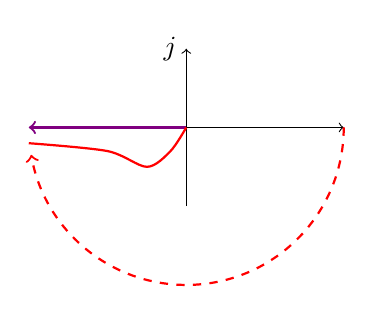
\begin{tikzpicture}[scale=1]
	\coordinate (o) at (0,0);
	\coordinate (ox) at (2,0);
	\draw[->] (-2,0) -- (ox);
	\draw[->] (0,-1) -- (0,1);
	\draw[->,violet,thick] (0,0) -- (-2,0); % -1/N(A)=-A\pi/4
	\draw [red,thick,smooth] plot coordinates {(-2,-0.2)(-1,-0.3)(-0.5,-0.5) (-0.2,-0.3) (0,0) }; %G(s)=(1+s)/s^2
	\draw[->,red,dashed,thick] (2,0) arc (0:-170:2);
	\draw (0,1) node[left] {$j$};
	\end{tikzpicture}
	
	G(s)的Nyquist曲线未包围或相交$\frac{-1}{N(A)}$曲线,系统稳定,不存在自振。
}

\onlytest{\newpage}

\question(20分)单位负反馈控制系统开环传递函数,
$$G(s)=\frac{20}{s(s+1)(s+5)}$$
串联校正网络:
$$G_c(s)=k\cdot\frac{T_b s+1}{bT_b s+1}\cdot\frac{aT_a s+1}{T_a s+1}$$
求解参数 $b,a,T_a$ 使校正后系统截止频率不变,稳态性能不变,相角裕度提高约 $30^\circ$ 。(已知 $0<b<1,\frac{1}{T_b}\approx 0$)

\onlyanswer
{
	答:利用迟后超前校正方法求解。
	计算校正前截止频率:
	\begin{align*}
	|G(s)| &=1 \\
	\omega_c &=2 
	\end{align*}
	计算超前校正网络参数:
	\begin{align*}
	\angle (2T_b j+1)-\angle(2bT_bj +1)&=30^{\circ} \\
	90^{\circ}-\angle(2bT_bj +1)&=30^{\circ} \\
	\angle (2bT_bj +1) &=60^{\circ} \\
	2bT_b &= \sqrt{3}\\
	b &= \frac{\sqrt{3}}{2T_b}
	\end{align*}
	由系统稳态性能不变可得: $k=1$ 。
	由迟后超前网络特性可得: $aT_a \geq T_b$ ,取 $aT_a=T_b$ 。
	由截止频率保持不变可得:
	\begin{align*}
	\frac{1}{b}\cdot a &= 1 \\
	a &= \frac{\sqrt{3}}{2T_b} \\
	T_a &= \frac{2T_b^2}{\sqrt{3}}
	\end{align*}
}

\question(20分)已知控制系统结构图如下所示:

\begin{tikzpicture}[node distance=3em,auto,>=latex', thick]
%\path[use as bounding box] (-1,0) rectangle (10,-2); 
\tikzstyle{block} = [draw,rectangle,thick,minimum height=1em,minimum width=1em]
\tikzstyle{sum} = [draw,circle,inner sep=0mm,minimum size=2mm]
\tikzstyle{branch} = [circle,fill,inner sep=0pt,minimum size=1mm]
\tikzstyle{connector} = [->,thick]

\def\r{\node(r){$r(t)$};}
\def\b(#1){\node[branch](b#1){};}
\def\p(#1){\node[sum](p#1){};}
\def\gc{\node[block](gc){$G_c(s)$};}
\def\gr{\node[block](gr){$G_r(s)$};}
\def\gp{\node[block](gp){$G(s)$};}
\def\g(#1){\node[block](g#1){$1$};}
\def\c{\node(c){$c(t)$};}

\matrix[ampersand replacement=\&, row sep=1em, column sep=2em]{
	\&         \&   \gr  \\
	\r  \&   \b(r)  \& \p(e)  \& \gc \& \p(r) \& \gp \& \b(c)  \& \c  \\
	\&         \&         \& \g(h)    \\
};
\draw [connector](r) -- (pe) ; 
\draw [connector](br) |- (gr) ; 
\draw [connector](gr) -| (pr) ; 
\draw [connector](pe) -- node[midway]{$E(s)$} (gc) ; 
\draw [connector](gc) -- (pr) ; 
\draw [connector](pr) -- (gp) ; 
\draw [connector](gp) -- (c) ; 
\draw [connector](bc) |- (gh) ; 
\draw [connector](gh) -| node[near end , left]{$-$} (pe) ; 
\end{tikzpicture} 

已知
\begin{align*}
G(s) &=\frac{1}{s+1} \\
G_c(s) &=1\\
G_r(s) &=\frac{k_1 s+k_2}{10s+1}\\
r(t)&=t\qquad(t>0)
\end{align*} 
当 $k_1=1,k_2=1$时,计算稳态误差;为使稳态误差为零,求解 $k_1,k_2$ 。

\onlyanswer
{
	答:
	$k_1=1,k_2=1$ 时,
	\begin{align*}
	\frac{E(s)}{R(s)} &= (1-\frac{s+1}{10s+1}\cdot\frac{1}{s+1})\frac{1}{1+\frac{1}{s+1}} \\
	&=\frac{10s^2+11s+1-(s+1)}{(s+2)(10s+1)} \\
	&=\frac{10s^2+(11-1)s}{(s+2)(10s+1)} \\
	E(s) &=\frac{10s^2+(11-1)s}{(s+2)(10s+1)} \cdot R(s) \\
	&=\frac{10s^2+10s}{(s+2)(10s+1)} \cdot \frac{1}{s^2} \\
	&=\frac{10s+10}{s(s+2)(10s+1)}\\
	\lim_{s\rightarrow 0} sE(s) &=5
	\end{align*}
	由 $G_r(s)=\frac{k_1 s+k_2}{10s+1}, r(t)=t, (t>0)$ ,得:
	\begin{align*}
	\frac{E(s)}{R(s)} &= (1-\frac{k_1s+k_2}{10s+1}\cdot\frac{1}{s+1})\frac{1}{1+\frac{1}{s+1}} \\
	&=\frac{10s^2+11s+1-(k_1s+k_2)}{(s+2)(10s+1)} \\
	&=\frac{10s^2+(11-k_1)s+(1-k_2)}{(s+2)(10s+1)} \\
	\end{align*}
	所以,当 $k_1=11,k_2=1$ 时,
	\begin{align*}
	E(s) &=\frac{10s^2+(11-k_1)s+(1-k_2)}{(s+2)(10s+1)}\cdot R(s) \\
	&=\frac{10s^2}{(s+2)(10s+1)}\cdot \frac{1}{s^2} \\
	&=\frac{1}{(s+2)(10s+1)} \\
	e_{ss} &= \lim_{s\rightarrow 0} sE(s) \\
	&= 0
	\end{align*}
	
}


\onlytest{\newpage}

\question(20分)已知控制系统结构图如下所示:

\begin{tikzpicture}[node distance=3em,auto,>=latex', thick]
%\path[use as bounding box] (-1,0) rectangle (10,-2); 
\tikzstyle{block} = [draw,rectangle,thick,minimum height=1em,minimum width=1em]
\tikzstyle{sum} = [draw,circle,inner sep=0mm,minimum size=2mm]
\tikzstyle{branch} = [circle,fill,inner sep=0pt,minimum size=1mm]
\tikzstyle{connector} = [->,thick]

\def\r{\node(r){$r(t)$};}
\def\rd{\node(rd){$r^*(t)$};}
\def\b(#1){\node[branch](b#1){};}
\def\p(#1){\node[sum](p#1){};}
\def\s(#1){\path[->] node[minimum size=2em] (s#1) {}; \draw (s#1.west)--(s#1.north east);\draw[->] (s#1.north west) arc (70:0:1.7em);\draw (s#1.south) node {$T$};}
\def\sd(#1){\path[->] node[minimum size=2em] (sd#1) {}; \draw[dashed] (sd#1.west)--(sd#1.north east);\draw[dashed,->] (sd#1.north west) arc (70:0:1.7em);\draw[dashed] (sd#1.south) node {$T$};}
\def\gc{\node[block](gc){$\dfrac{k}{s}$};}
\def\gd{\node[block](gd){$\dfrac{k}{s}$};}
\def\g(#1){\node[block](g#1){$1$};}
\def\ed{\node(ed){$e^*(t)$};}

\matrix[ampersand replacement=\&, row sep=1em, column sep=2em]{
	\&         \&   \& \g(ch)    \\
	\r  \&   \b(r)  \& \p(ce)  \& \gc  \& \b(c)  \& \p(e)   \&  \s(e)  \& \ed  \\
	\&  \p(de) \& \s(de)  \& \gd  \& \& \b(d)    \\  
	\&         \&   \& \g(dh)    \\
};
\draw [connector](r) -- (pce) ; 
\draw [connector](r) -| (pde) ; 
\draw [connector](pce) -- (gc) ; 
\draw [connector](gc) -- (pe) ; 
\draw [connector](bc) |- (gch) ; 
\draw [connector](gch) -| node[near end , left]{$-$} (pce) ; 
\draw [](pde) -- (sde) ;
\draw [connector](sde) -- (gd) ;  
\draw [connector](gd) -| node[near end , left ]{$-$} (pe) ; 
\draw [connector](bd) |- (gdh) ; 
\draw [connector](gdh) -| node[near end , left ]{$-$} (pde) ; 
\draw [](pe)  -- (se) ; 
\draw [connector](se) -- (ed) ; 
\end{tikzpicture} 

当$r(t)=1,(t>0)$时,求解 $e(nT)$,并分析使系统稳定的 $k$ 取值范围。 

常见 $Z$ 变换表:
$$
\begin{array}{ccc}
f(t)     &   F(s)  &  F(Z)   \\ 
\delta(t)   &   1      &  1    \\  
1(t)         &   \frac{1}{s} &  \frac{1}{1-z^{-1}}   \\ 
t            &   \frac{1}{s^2} &  \frac{Tz^{-1}}{(1-z^{-1})^2}   \\  
e^{-at}      &   \frac{1}{s+a} &  \frac{1}{1-e^{-aT}z^{-1}}  \\ 
a^{t/T}      &   \frac{1}{s-(1/T)\ln a} & \frac{1}{1-az^{-1}} 
\end{array}
$$

\onlyanswer
{
	答:由结构图可知:
	\begin{align*}
	R(s) &= \frac{1}{s} \\
	E^*(s) &= \left[\frac{\frac{k}{s}}{1+\frac{k}{s}}R(s)\right]^*-\frac{[\frac{k}{s}]^*}{1+[\frac{k}{s}]^*}R^*(s) \\
	&= \left[\frac{k}{s(s+k)}\right]^* -\frac{[\frac{k}{s}]^*}{1+[\frac{k}{s}]^*}R^*(s) \\
	&= \left[\frac{1}{s}-\frac{1}{s+k}\right]^* -\frac{[\frac{k}{s}]^*}{1+[\frac{k}{s}]^*}R^*(s) \\
	E(z)  &=\frac{1}{1-z^{-1}}-\frac{1}{1-e^{-kT}z^{-1}}-\frac{\frac{k}{1-z^{-1}}}{1+\frac{k}{1-z^{-1}}}\frac{1}{1-z^{-1}} \\
	&=\frac{1}{1-z^{-1}}-\frac{1}{1-e^{-kT}z^{-1}}-\frac{k}{1+k-z^{-1}}\frac{1}{1-z^{-1}} \\
	&=\frac{1}{1-z^{-1}}-\frac{1}{1-e^{-kT}z^{-1}}-\frac{1}{1-z^{-1}}+\frac{1}{1+k-z^{-1}} \\
	&=-\frac{1}{1-e^{-kT}z^{-1}}+\frac{1}{1+k-z^{-1}} \\
	e(nT) &=-e^{-nkT}+\left[\frac{1}{1+k}\right]^{n+1}
	\end{align*}
	由 $e(nT)$ 表达式可知,当 $k\in(0,\infty)$ 时系统稳定。
}


\question(20分){已知控制系统结构图如下所示, 已知$r(t)=1,(t>0)$ 求解当$a=0$  时的 $Y(z)$ 与 $a\in(0,1]$ 时的 $Y(z)$ 。

\begin{tikzpicture}[node distance=3em,auto,>=latex', thick]
%\path[use as bounding box] (-1,0) rectangle (10,-2); 
\tikzstyle{block} = [draw,rectangle,thick,minimum height=1em,minimum width=1em]
\tikzstyle{sum} = [draw,circle,inner sep=0mm,minimum size=2mm]
\tikzstyle{branch} = [circle,fill,inner sep=0pt,minimum size=1mm]
\tikzstyle{connector} = [->,thick]

\def\r{\node(r){$r(t)$};}
\def\rd{\node(rd){$r^*(t)$};}
\def\b(#1){\node[branch](b#1){};}
\def\p(#1){\node[sum](p#1){};}
\def\s(#1){\path[->] node[minimum size=2em] (s#1) {}; \draw (s#1.west)--(s#1.north east);\draw[->] (s#1.north west) arc (70:0:1.7em);\draw (s#1.south) node {$T$};}
\def\sd(#1){\path[->] node[minimum size=2em] (sd#1) {}; \draw[dashed] (sd#1.west)--(sd#1.north east);\draw[dashed,->] (sd#1.north west) arc (70:0:1.7em);\draw[dashed] (sd#1.south) node {$T$};}
\def\ga{\node[block](g1){$\dfrac{1}{s+1}$};}
\def\gb{\node[block](g2){$e^{-asT}$};}
\def\c{\node(c){$y(t)$};}
\def\cd{\node(cd){$y^*(t)$};}
\def\g(#1){\node[block](g#1){$1$};}

\matrix[ampersand replacement=\&, row sep=1em, column sep=2em]{
	\&         \& \sd(r)  \& \rd      \&  \&     \&          \&    \&  \\
	\r  \& \b(r)   \& \p(e)   \& \s(e) \& \ga \&  \b(c)  \&  \gb \&  \s(c) \& \cd \\
	\&         \& \           \& \g(h) \\
};
\draw [connector](r) -- (pe) ; 
\draw [dashed](br)  |- (sdr) ; 
\draw [connector,dashed](sdr) -- (rd) ; 
\path[](pe) edge node[midway] {$e(t)$} (se) ; 
\draw [connector] (se) -- node[midway] {$e^*(t)$} (g1); 
\draw [connector] (g1) -- node[midway] {$   $} (g2); 
%\draw [connector] (g2)-- (sc); 
\path[](g2) edge node[midway] {$y(t)$} (sc) ; 
\draw [connector] (sc)-- (cd); 
%\draw [dashed](bc)  |- (sdc) ; 
%\draw [connector,dashed](sdc) -- (cd) ; 
\draw [connector](bc)  |- (gh) ; 
\draw [connector](gh) -|  node[near end,left]{$-$} (pe) ; 
\end{tikzpicture} 

\onlyanswer
{
	答:$a=0$ 时:
	
	\begin{align*}
	Y^*(s) &= \frac{[\frac{1}{s+1}]^*}{1+[\frac{1}{s+1}]^*}R^*(s) \\
	Y(z)  &= \frac{\frac{1}{1-e^{-T}z^{-1}}} {1+\frac{1}{1-e^{-T}z^{-1}}}\cdot\frac{1}{1-z^{-1}} \\
	&= \frac{1}{(2-e^{-T}z^{-1})(1-z^{-1})} 
	\end{align*}
	
	
	
	$a\in(0,1]$时:
	
	
	\begin{align*}
	Y^*(s) &= \left[\frac{e^{-aTs}}{s+1}\right]^*\frac{R^*_T(s)}{1+[\frac{1}{s+1}]^*} \\
	Y(z)  &={\cal Z}\left[\left[\frac{e^{-aTs}}{s+1}\right]^*\right]\cdot \frac{1}{1+\frac{1}{1-e^{-T}z^{-1}}}\cdot \frac{1}{1-z^{-1}} \\
	&=\frac{e^{aT}e^{-T}z^{-1}}{1-e^{-T}z^{-1}}\cdot \frac{1}{1+\frac{1}{1-e^{-T}z^{-1}}}\cdot \frac{1}{1-z^{-1}} \\
	&=\frac{e^{aT}e^{-T}z^{-1}}{(1-z^{-1})(2-e^{-T}z^{-1})}
	\end{align*}
	其中:
	\begin{align*}
	\frac{e^{-aTs}}{s+1} &= {\cal L}[e^{-(t-aT)}]\qquad (t\geq aT)  \\
	{\cal Z}[e^{-nT+aT} ] &= \sum_{n=1}^{\infty} e^{-nT+aT}z^{-n}\\
	&=\frac{e^{aT-T}z^-1}{1-e^{-T}z^-1}
	\end{align*}
}

}

%\onlytest{\vskip 3em}

%\onlytest{\newpage}



